\documentclass[11pt]{article}
\usepackage[margin=1in]{geometry}
\usepackage[T1]{fontenc}
\usepackage[utf8]{inputenc}
\usepackage{lmodern}
\usepackage{booktabs}
\usepackage{tabularx}
\usepackage{graphicx}
\usepackage{amsmath}
\usepackage{amssymb}
\usepackage{enumitem}
\usepackage{microtype}
\usepackage[hidelinks]{hyperref}
\usepackage[numbers,sort&compress]{natbib}

\emergencystretch=2em
\setlist{itemsep=2pt,topsep=4pt}
\newcommand{\code}[1]{\texttt{#1}}

\title{The Gateway Is Not the Platform:\\
Porting a Cloud-Native Memory System On-Premises}

\author{Kostadis Roussos\\
Independent researcher\\
\texttt{kostadis@gmail.com}}

\date{October 25, 2026}

\begin{document}
\maketitle

\begin{abstract}
We ported Cognee, an open-source knowledge-graph memory library built against hosted model APIs, to
a two-node NVIDIA DGX Spark cluster serving open-weight models through vLLM and Ollama. The workload
was a real 106-file tabletop-campaign corpus of about 55,000 words.

Pointing Cognee at an OpenAI-compatible endpoint took minutes, and a one-document smoke test passed.
The full ingest then failed on roughly six attempts across one day, each in a different way:
\begin{itemize}
  \item unbounded fan-out against a fixed number of serving slots;
  \item client timeouts that counted queue wait, causing retry storms;
  \item retry layers that multiplied a 600\,s timeout into 1,801\,s;
  \item all-or-nothing durability that discarded 50 minutes of work;
  \item no liveness signal on any of three dependencies.
\end{itemize}

A later version completed the same corpus in 27 minutes. A third run on a reasoning model failed
again: the model spent its whole output budget thinking and wrote nothing, and the downstream
timeouts and rate limiting were symptoms. A second system, the MemPalace semantic memory store,
needed about a dozen changes before it ran against a local embedder.

We argue three things:
\begin{enumerate}
  \item Cloud-built tools inherit a control plane they never see: elastic capacity, admission,
    liveness, and per-model behavior.
  \item An API-compatible gateway restores the wire protocol but not those semantics, so it is
    necessary but insufficient.
  \item On-premises AI is mostly the work of building, and adapting tools to, a local control plane
    that states capacity, model behavior, and configuration authority explicitly.
\end{enumerate}
\end{abstract}

\section{Introduction}
\label{sec:intro}

The usual story of on-premises AI is about models: which open-weight model fits in memory, how fast
it decodes, and how close its quality comes to a frontier API. That story assumes the rest of the
stack carries over. Once a local server speaks the OpenAI chat-completions protocol, the libraries
built on that protocol should work.

They connect. They do not necessarily work. A hosted model API is more than an endpoint. Behind it
sits a control plane the client never sees:
\begin{itemize}
  \item it admits requests elastically, so fan-out width is someone else's problem;
  \item it answers in seconds, so a timeout measures failure, not queue depth;
  \item it is always up, so the only health check needed is ``did the call return'';
  \item its models behave as documented, so an output budget means output.
\end{itemize}
Libraries built against that API never needed to model any of this, so they don't.

This paper reports what happened when we moved one such library, Cognee~\cite{cognee}, onto two DGX
Spark boxes. We also draw on a second system, MemPalace~\cite{mempalace}, ported in parallel. We make
three claims:
\begin{enumerate}
  \item \textbf{Cloud assumptions are diffuse.} They are not in one adapter. They are spread across
    timeouts, retries, concurrency, durability, health checks, configuration loading, and the
    embedded databases. Fixing one exposed the next.
  \item \textbf{A gateway is necessary but insufficient.} An OpenAI-compatible endpoint, and a
    router such as LiteLLM in front of it, restores the wire protocol. It does not restore
    admission, liveness, or per-model behavior. Worse, it makes the local server look like the
    cloud to code that branches on provider type.
  \item \textbf{On-premises AI is control-plane work.} What made the systems run was not a better
    model. It was a local control plane that states what the cloud left implicit: serving
    capacity, per-model behavior, and a single authority for configuration.
\end{enumerate}
The evidence is one operator, one corpus, and two systems. Section~\ref{sec:related} discusses what
that does and does not support.

\section{Background}
\label{sec:background}

\subsection{Hardware and serving}

The cluster is two NVIDIA DGX Spark boxes (GB10, 128\,GB of unified CPU/GPU memory, about
273\,GB/s of memory bandwidth). Each serves one chat model through vLLM's OpenAI-compatible API.
Its batch width is fixed by \code{max\_num\_seqs}, which we ran at 3, 8 or 16 depending on the
configuration.

Embeddings come from Ollama serving \code{qwen3-embedding:0.6b} (1024 dimensions). Decode is
bandwidth-bound, so a long structured output is the most expensive thing a client can ask for.

The chat models varied across the study. The first runs (2026-07-04) used
Qwen3-Next-80B-A3B-Instruct-FP8. The August retest used DeepSeek-V4-Flash-DSpark across both boxes.
The September retest used the reasoning model \code{qwen3.8-flash-next}.

\subsection{Cognee}

Cognee builds a knowledge graph from documents and answers questions over it. \code{remember()}
runs \code{add()} (store raw text), then \code{cognify()} (all the LLM work), then an optional
self-improvement loop, which we disabled.

For each document, \code{cognify()} classifies the document, chunks it, and runs
\code{extract\_graph\_\allowbreak and\_summarize}: two structured-output chat calls per chunk, one for the graph
and one for the summary. It then embeds the results and writes them to three embedded stores:
\begin{itemize}
  \item \textbf{Graph:} Kuzu, wrapped as ``Ladybug'' and run as a subprocess.
  \item \textbf{Vectors:} LanceDB.
  \item \textbf{Metadata:} SQLite.
\end{itemize}
Cognee reaches the model through LiteLLM and enforces output structure through Instructor.

\subsection{Workload}

The corpus is the grounding documents of a running tabletop campaign: three or four dense state
documents of 2,000 to 4,800 words each, plus 103 or 104 NPC dossiers of about 230 words each. That is
106 to 108 files and about 50,000 to 55,000 words. A single dense document produces
graph-extraction outputs of thousands of tokens per chunk.

\section{Deployment}
\label{sec:deployment}

\subsection{Wiring}
\label{sec:wiring}

Connecting Cognee to the local stack was easy, and that ease is what misleads. Five settings in
\code{.env} did it:
\begin{itemize}
  \item \code{LLM\_PROVIDER="custom"}, which routes through LiteLLM;
  \item an \code{openai/}-prefixed model id, which LiteLLM needs to route to \code{LLM\_ENDPOINT} and
    strips before sending;
  \item the vLLM endpoint;
  \item \code{EMBEDDING\_PROVIDER="openai\_compatible"}, pointed at Ollama's \code{/v1};
  \item \code{EMBEDDING\_DIMENSIONS="1024"}.
\end{itemize}

A one-document smoke test then passed: \code{party.md}, about 1,400 words, 4 LLM calls, 0 retries,
202\,s, 61 nodes and 140 edges, and a correct recall answer.

Three configuration traps had already appeared, each a silent failure:
\begin{enumerate}
  \item \code{import cognee} calls \code{load\_dotenv(override=True)}, so environment variables set in
    Python before the import are overwritten. One run meant for spark2 ran on spark1, and its
    measurements were mislabeled.
  \item \code{.env} is resolved relative to the working directory. From another directory, Cognee
    falls back to OpenAI defaults and fails with an authentication error that names the wrong
    cause.
  \item The \code{ollama} embedding provider requires \code{transformers} and a Hugging Face
    tokenizer download. \code{openai\_compatible} falls back to TikToken.
\end{enumerate}
None of these is a bug in isolation. Each assumes that configuration has one obvious home, and on a
multi-box local network it doesn't.

\subsection{Calibration}

On a single document the workload is decode-bound: the two graph-extraction calls took 97.5\,s and
94.5\,s of the 202\,s. At batch scale we measured aggregate decode on the real extraction load under
three vLLM configurations (Qwen3-Next-80B, spark2), shown in Table~\ref{tab:calibration}.

\begin{table}[t]
\centering
\caption{Aggregate and per-stream decode on the real graph-extraction load (Qwen3-Next-80B, spark2).}
\label{tab:calibration}
\begin{tabular}{lrrr}
\toprule
Configuration & Slots & Aggregate (tok/s) & Per stream (tok/s) \\
\midrule
MTP-2 speculative decode & 3 & 92 & 30.7 \\
Plain decode & 16 & 125 & 7.8 \\
MTP-2 speculative decode & 8 & 138 & 17.3 \\
\bottomrule
\end{tabular}
\end{table}

Speculative decoding accepted 86 to 93\% of draft tokens on the rigid graph JSON, against about 77\%
on code. That made each MTP stream about 2.3 times faster than a plain one. Eight fast streams beat
sixteen bandwidth-contended ones. Prefix caching was immaterial: we measured a hit rate near 0\%,
and the cacheable prefix was under 3\% of a decode-bound call.

This was the study's cleanest result, and it is a result about the server.
Section~\ref{sec:broke} is about the client.

\section{Where cloud assumptions broke}
\label{sec:broke}

\subsection{Six attempts, six failures (Cognee 1.2.2, 2026-07-03 to 07-04)}

Table~\ref{tab:attempts} lists the attempts in order.

\begin{table}[t]
\centering
\caption{Six attempts to ingest the full corpus with Cognee 1.2.2, 2026-07-03 to 07-04.}
\label{tab:attempts}
\small
\begin{tabularx}{\textwidth}{>{\raggedright\arraybackslash}p{0.27\textwidth}
                             >{\raggedright\arraybackslash}X
                             >{\raggedright\arraybackslash}X}
\toprule
Attempt & Outcome & Cause \\
\midrule
Latency box (MTP-2, 3 slots), overnight & Died after 3\,h 12\,min; 253 timeouts &
  About 39 concurrent requests on a 3-slot queue; retry storm \\
Throughput box (plain, 16 slots) & Wedged mid-run & One hung request, no liveness signal \\
MTP-2, 8 slots & Clean for about 50\,min, then crashed &
  Queue-tail requests timed out while waiting, and their retries deepened the queue \\
Batched \code{remember()} of 6 documents & First batch ran 61\,min, then failed &
  The four dense documents landed together; retry churn \\
One document at a time, OS \code{timeout 600} & Small documents done; dense ones killed &
  A dense document needs over 10\,min of extraction alone \\
Same, with a 1,800\,s timeout & Extraction finished in about 10\,min, then wedged &
  The hang moved to the graph-persist phase \\
\bottomrule
\end{tabularx}
\end{table}

Every fix exposed the next failure. That pattern is our main evidence that the cloud assumptions are
diffuse.

\subsection{The failure modes}
\label{sec:failure-modes}

\begin{enumerate}
  \item \textbf{Unbounded fan-out.} Documents are gated by a semaphore of 20, but the per-chunk calls
    inside a document run under a bare \code{asyncio.gather} with no cap. That gave about 40 to 48
    concurrent requests, so vLLM's \code{max\_num\_seqs} was the only throttle in the system: 3 to 15
    times overcommitted~\cite{cognee3870}.
  \item \textbf{Timeouts that count queue wait.} The client timer starts at send. A request that is
    alive but waiting in a deep queue times out, is retried, and the retry joins the same queue. On
    a cloud API queue wait is near zero, so this coupling is invisible.
  \item \textbf{Multiplied retry layers.} LiteLLM retries internally, and Instructor retries on top.
    A 600\,s timeout surfaced after 1,801\,s, and 1,800\,s after 5,401\,s. A smaller timeout does
    not fail faster.
  \item \textbf{All-or-nothing durability.} One straggler's \code{InstructorRetryException}
    propagated through the gather and aborted \code{remember()}. Fifty minutes of extraction
    produced an empty graph. There was no checkpoint.
  \item \textbf{No liveness signal.} The only health check is a one-shot 30\,s preflight at startup.
    Non-streaming structured output gives the client no way to tell ``slow'' from ``hung''.
  \item \textbf{The assumption spans every dependency.} Stalls appeared on the chat path, the
    embedding path, and the graph-persist path. In the final wedge the main process sat in
    \code{epoll\_wait} while the Kuzu subprocess workers sat in \code{pipe\_read}, with no progress.
\end{enumerate}

We first attributed the persist hang to a known orphaned-lock issue~\cite{cognee3708}. A later
investigation showed that attribution was wrong: the issue concerned a different race, and its
crash reproducer did not reproduce here. Kuzu operations are serialized by design. So persist time
across concurrently admitted documents adds up rather than overlaps, which can look like a hang
without being one.

\subsection{The retest that succeeded (2026-08-01)}

On current Cognee \code{main}, the same corpus completed:
\code{status='completed', items=106, elapsed=1636.3s}, about 27 minutes, with zero errors and zero
retries. All five evaluation questions came back correct and grounded in the source.

The backend had also changed, to DeepSeek-V4-Flash-DSpark, so this is not a single-variable
comparison. Upstream had meanwhile added a backend-aware overload policy and hardened its database
workers.

\subsection{The retest that failed again (2026-09-10)}
\label{sec:retest-failed}

Against a reasoning model the same recipe broke in a new way. Cognee allowed 16,384 output tokens
per call. The model spent all of them thinking and wrote nothing.

On a 4,000-character input, thinking on took 251\,s and produced 0 characters; thinking off took
172\,s and produced 25,397. The empty answers then produced 493 timeouts. Cognee's automatic rate
limiter reacted to those timeouts by slowing the run further, and the retries added load.

About five GPU-hours went into tuning those four symptoms before the cause was found. Disabling
thinking through \code{LLM\_ARGS} fixed it: zero timeouts, 104 items, 26.8 minutes.

The same retest found that a file path outside \code{COGNEE\_ALLOWED\_LOCAL\_FILE\_ROOTS} is ingested
as literal text, and \code{remember()} still reports \code{completed}. A small smoke-test file hid
both problems.

\section{The gateway: necessary but insufficient}
\label{sec:gateway}

By \emph{gateway} we mean the compatibility layer that makes a local server answer like a hosted
one. Here that was vLLM's and Ollama's OpenAI-compatible endpoints plus LiteLLM routing. The same
reasoning applies to a proxy or router placed in front of them.

\begin{figure}[!htb]
\centering
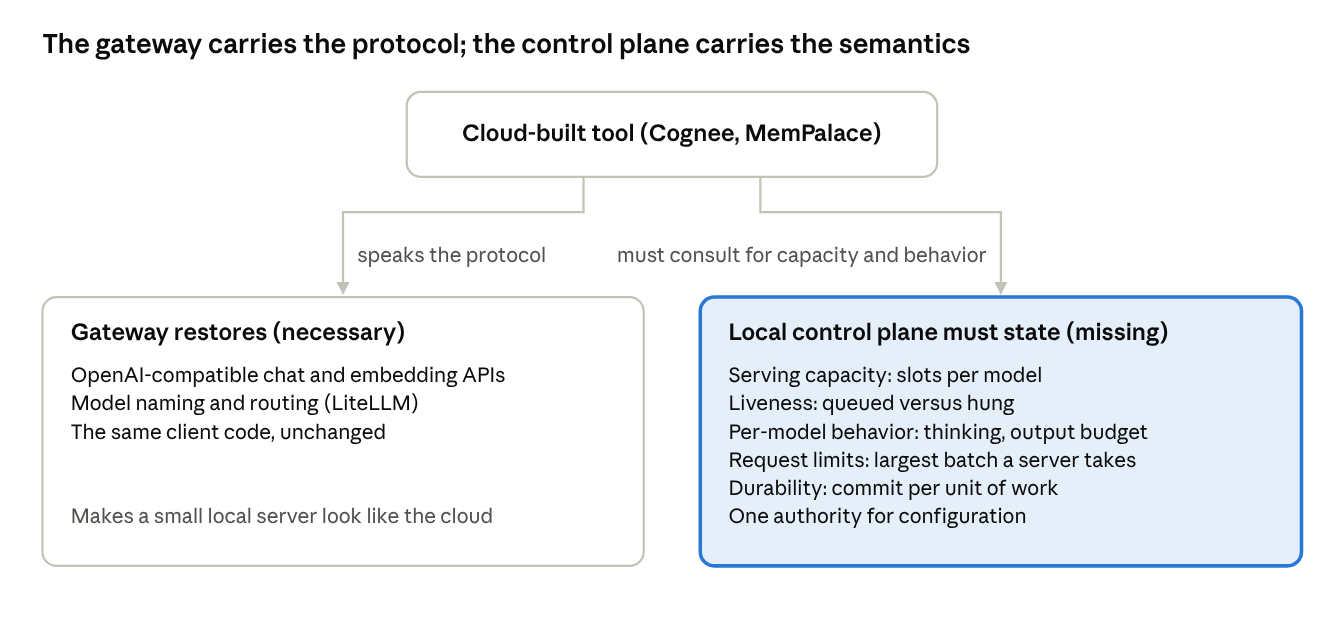
\includegraphics[width=0.85\textwidth]{gateway-not-platform-diagram.png}
\caption{Gateway versus local control plane.}
\label{fig:gateway}
\end{figure}

Figure~\ref{fig:gateway} shows the split. The tool reaches the model through the gateway. Everything
in the right-hand box, the cloud supplied implicitly, and on-premises nothing does unless someone
builds it.

\subsection{Why it is necessary}

Without the gateway, nothing connects. With it, Cognee and MemPalace both reached local models
through configuration alone, with no code changes. Every later step depended on that.

\subsection{Why it is insufficient}

A gateway carries the protocol. It does not carry the properties the client built on that protocol
depends on. We saw five kinds of gap.

\paragraph{Capacity is not in the protocol.} Nothing in a chat-completions response says ``you are
request 41 for 8 slots''. The client cannot see queue depth, so it cannot tell a slow request from a
dead one, and its timeouts and retries react to the wrong signal.

\paragraph{The gateway disguises locality.} Cognee decides whether a provider is local by its name.
Ollama and llama.cpp get a local rate-limit default of 10 requests per minute. vLLM is deliberately
excluded, and the code comment says it ``absorbs concurrency like a cloud endpoint''. That is true
of a large vLLM deployment and false of one box with 8 slots. The more faithfully the gateway
imitates the cloud, the more surely downstream code treats the server as cloud.

\paragraph{Admission control at the gateway paced the wrong thing.} We tested a requests-per-minute
limiter, and later Cognee's automatic one. Both made the run worse. They pace how often requests
start, while the constraint is how many are in flight, and they reacted to timeouts that were
symptoms of something else (\S\ref{sec:retest-failed}). Admission belongs to whoever knows
capacity, and the gateway does not.

\paragraph{Model behavior and request limits pass through unchanged.} Whether a model thinks before
answering, and how much of an output budget that consumes, is a per-model fact. Whether a server
survives a 1,000-input embedding request is a per-server fact. MemPalace sent such batches to
Ollama's compatible \code{/api/embed}, and Ollama's model runner crashed on large files (MemPalace
\#57~\cite{mempalace}). The fix was client-side sub-batching to 64.

\paragraph{Some dependencies sit behind no gateway at all.} Cognee's graph store is an embedded Kuzu
subprocess, and its configuration is a \code{.env} file loaded relative to the working directory with
override semantics. No proxy in front of the model touches either.

\section{Discussion: building a local control plane}
\label{sec:discussion}

What made our tools run on the Spark was not a better model or a better gateway. It was a set of
small, explicit authorities that state what the cloud keeps implicit. We built three of them while
working on these systems.

\subsection{What the local control plane holds}

\begin{itemize}
  \item \textbf{Per-model behavior: a model registry.} \code{dgxlib} (in the \code{dgx-fun}
    repo~\cite{dgxfun}) keeps a registry keyed by model id: whether the model can think, whether
    thinking is on by default, its read timeout, and its concurrency. A call site states its intent
    (``no thinking for this extraction''), and the registry decides whether the model can honor it.
    Swapping a model becomes a one-line registry edit. The failure in \S\ref{sec:retest-failed} is
    exactly the fact this registry exists to hold.
  \item \textbf{Capacity.} The registry exposes per-model serving concurrency, so a client can size
    its fan-out to the slots that exist instead of discovering them through timeouts.
  \item \textbf{Configuration authority.} On the mining host, one hand-edited file
    (\code{hypostasis.yaml}) declares the vector backend, embedding provider, model and endpoint.
    Every component's config is rendered from it. That rules out the class of bug in
    \S\ref{sec:wiring}, where two loaders disagree about which endpoint is real.
\end{itemize}

\subsection{What tools must do with it}

The control plane only helps tools that consult it. From our failures, a tool that is meant to run
anywhere other than a hosted API should:
\begin{enumerate}
  \item \textbf{Bound fan-out from declared capacity}, not from a semaphore on documents.
  \item \textbf{Time from progress, not from send.} Streaming with an idle-token timeout, as
    \code{dgxlib}'s client does, distinguishes queued from hung.
  \item \textbf{Keep one retry layer} and own it.
  \item \textbf{Commit per unit of work}, so one straggler costs one document, not the run.
  \item \textbf{Treat model behavior as data} (thinking, output budget, structured-output support),
    looked up rather than assumed.
  \item \textbf{Fail loudly on silent fallbacks.} Ingesting a path as text, falling back to OpenAI
    defaults, and assuming a vector store's embedder identity should all be errors, not completions
    or warnings.
\end{enumerate}

\subsection{The same lesson in a second system}

MemPalace, a semantic memory store, needed about a dozen changes on our fork~\cite{mempalace} before
it ran against a local embedder:
\begin{itemize}
  \item remote embedding providers;
  \item a vector backend that does not import ChromaDB;
  \item per-palace scoping of every read and write;
  \item client-side sub-batching for Ollama.
\end{itemize}

Switching the embedding model itself was one line of configuration. Its logging still assumes the
cloud's single-machine shape: a warning about precomputed vectors fires on every mined file, and so
does an embedder-identity warning. The vector store does record an identity, but it records the
embedder function's name (\code{embed}) rather than the model, and the adapter never reads it. A
tool that cannot tell its normal path from an anomaly is another symptom of the missing control
plane.

\section{Related work and limitations}
\label{sec:related}

\subsection{Related work}

The failure modes in Section~\ref{sec:broke} are old distributed-systems problems in new clothes.
Timeouts that include queueing, layered retries that amplify load, and the need for per-unit
durability are standard lessons of large-service operation. Retry budgets, deadline propagation and
backpressure are their usual remedies. What is new is where they surface. LLM tooling grew up behind
provider APIs that absorbed these problems, so its libraries never adopted the remedies.

We have not run a systematic survey of other memory, RAG or agent frameworks, and we make no claim
about how common these patterns are. That survey is future work.

\subsection{Limitations}

\begin{itemize}
  \item \textbf{One operator, one corpus, two systems.} The evidence is a case study, not a
    benchmark.
  \item \textbf{Confounded comparisons.} The run that succeeded used a newer Cognee and a different
    chat model than the runs that failed. We cannot attribute the success to either change alone.
  \item \textbf{Hardware specificity.} The slot counts and decode rates are specific to GB10-class
    devices with about 273\,GB/s of memory bandwidth. A larger local cluster would hide some of
    these gaps the way the cloud does.
  \item \textbf{A corrected attribution.} Our first diagnosis of the persist hang cited the wrong
    upstream issue (\S\ref{sec:failure-modes}). We report the correction because the episode is
    itself evidence: without liveness signals, diagnosis falls back on inference.
\end{itemize}

\section{Conclusion}

Moving a cloud-built AI library on-premises is mostly not about the model. The model was the part
that worked: an 80B mixture-of-experts model decoding structured JSON at 138 tok/s across 8
speculative streams.

What failed was everything the library had assumed about who manages capacity, liveness, retries,
durability, model behavior and configuration. The cloud provides those through a control plane its
clients never see. An API-compatible gateway brings back the protocol, which is necessary for
anything to connect. It cannot bring back the control plane, and by imitating the cloud it can hide
the difference from the code that most needs to see it.

On-premises AI therefore needs two things the cloud never asked for. The first is a local control
plane that states capacity, per-model behavior and configuration authority explicitly. The second is
tools written to consult it.

\begin{thebibliography}{5}

\bibitem{cognee}
Cognee: open-source AI memory library.
\newblock \url{https://github.com/topoteretes/cognee}.

\bibitem{cognee3870}
Cognee issue \#3870: chat-layer robustness on local backends (fan-out, retry stacking, durability).
\newblock \url{https://github.com/topoteretes/cognee/issues/3870}.

\bibitem{cognee3708}
Cognee issue \#3708: orphaned Kuzu lock after a worker crash; open fixes PR \#4033 and PR \#4249.
\newblock \url{https://github.com/topoteretes/cognee/issues/3708}.

\bibitem{mempalace}
MemPalace fork, branch \texttt{kostadis-dev}; issues \#33, \#57 and \#59.
\newblock \url{https://github.com/kostadis/mempalace}.

\bibitem{dgxfun}
dgx-fun working notes: \texttt{cognee-local-control-plane-2026-07-04.md},
\texttt{cognee-local-control-plane-RETEST-2026-08-01.md}, \texttt{cognee-dgx-setup-guide.md},
\texttt{dgxlib/ARCHITECTURE.md}.

\end{thebibliography}

\end{document}
